\section{Library/Framework}
\textbf{Library} stellt bereits fertig implementierte Funktionalitäten zur Verfügung und der Benutzer kann diese normalerweise nicht überschreiben. Diese können über API aufrufe (aka Methoden aufrufe) genutzt werden zB \textit{std::abs(...)}, wobei std die Standard-Library von c++ ist. \textbf{Framework} bietet hingegen ein Gerüst an, welches vom Benutzer erweitert werden kann zB QT oder .NET. In der Umgangssprache sind diese zwei Begriffe äquivalent.
\begin{center}
	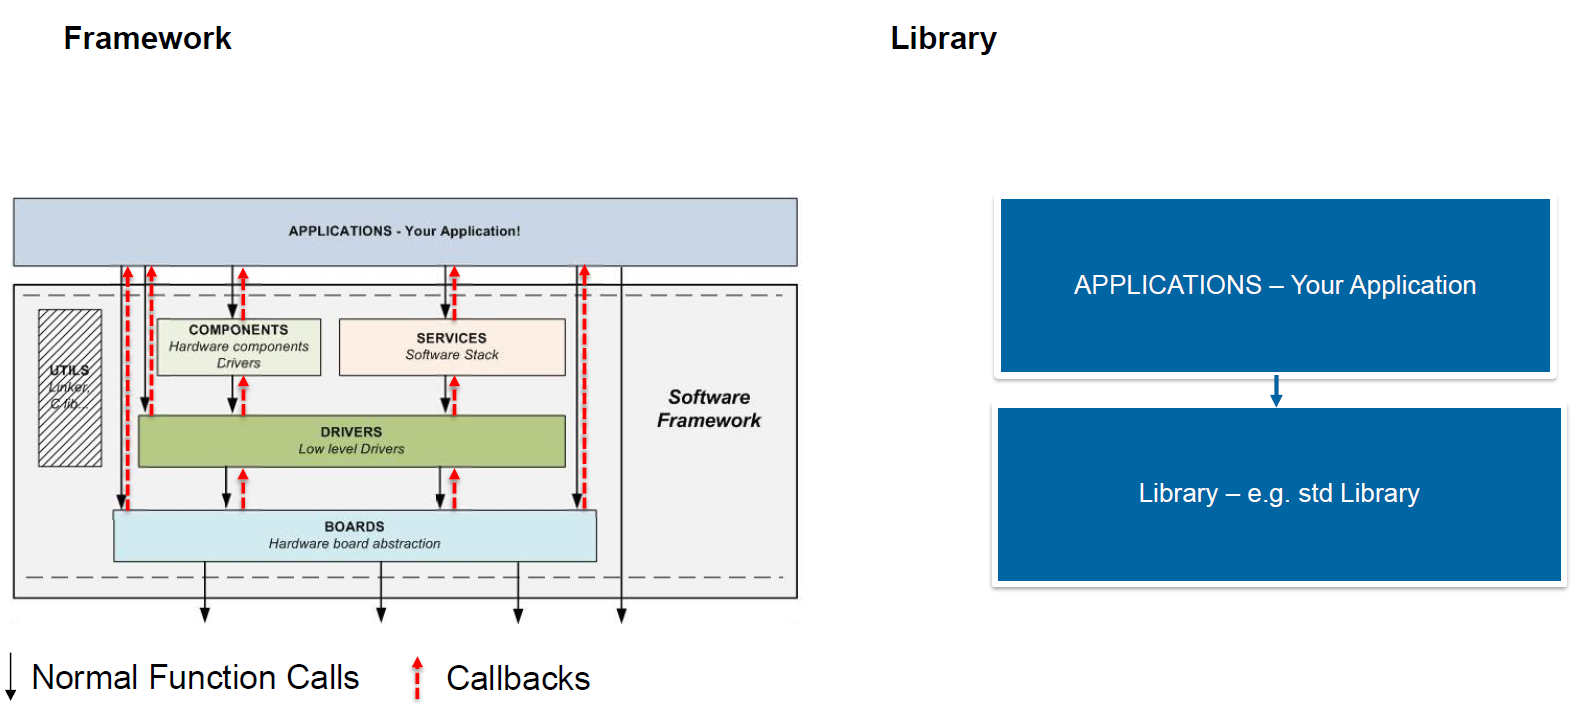
\includegraphics[width=\columnwidth]{Images/framework_library}
\end{center}


\subsection{Static vs Shared}
In c++ werden Klassen beim Kompilieren in Object Files umgewandelt. Eine Sammlung von Object-Files ergeben eine Library (Bibliothek) welche beim Linken Statisch oder als Shared hinzugefügt werden. Der Output hängt vom gewählten Target ab (im folgenden zB Windows). 

Jede \textbf{Shared-Library} endet auf Windows mit *.dll (Dynamic Link Library) und werden nach dem Programmstart geladen. Dies macht die *.exe sehr viel kleiner, wenn zB DLL zwischen Applikationen geteilt werden. Bei nicht vorhandenen DLL kann die Applikation jedoch nicht gestartet werden. Bei \textbf{Static-Library} werden die Object-Files direkt in die *.exe gelinkt, was diese grösser macht, jedoch müssen beim Programmstart nicht zusätzliche Libs geladen werden (bzw können nicht vergessen werden).